\documentclass[tikz,border=12pt]{standalone}
% Shared visual language for standalone EMT block diagrams.
\usepackage{amsmath}
\usetikzlibrary{arrows.meta,backgrounds,calc,fit,positioning}

\tikzset{
    emt diagram/.style = {>={Stealth[length=2.4mm]}},
    line/.style        = {semithick, rounded corners=6pt},
    block/.style       = {draw, semithick, fill=white,
                          minimum height=1cm, minimum width=2.3cm},
    hblock/.style      = {block, minimum width=2.24cm, minimum height=1.3cm},
    vblock/.style      = {block, minimum width=1.3cm, minimum height=2.24cm},
    sum/.style         = {draw, semithick, fill=white, circle,
                          inner sep=2.6pt},
    signal/.style      = {circle, fill, inner sep=1.4pt,
                          label distance=3pt},
    sig/.style         = {font=\small},
    pm/.style          = {font=\scriptsize},
    wire jump/.style   = {line,
                          preaction={draw=white, line width=3pt,
                                     line cap=round}},
    enclosure/.style   = {draw, dashed, semithick, rounded corners=4pt},
    operator enclosure/.style = {enclosure, inner xsep=7mm, inner ysep=6mm}
}


% TUNABLES: pulse-edge spacing, stack offsets, and output spacing.
\def\edgerow{1.2}
\def\stackstep{0.22}
\def\stackfar{0.8}
\def\outputrow{1.05}

\begin{document}
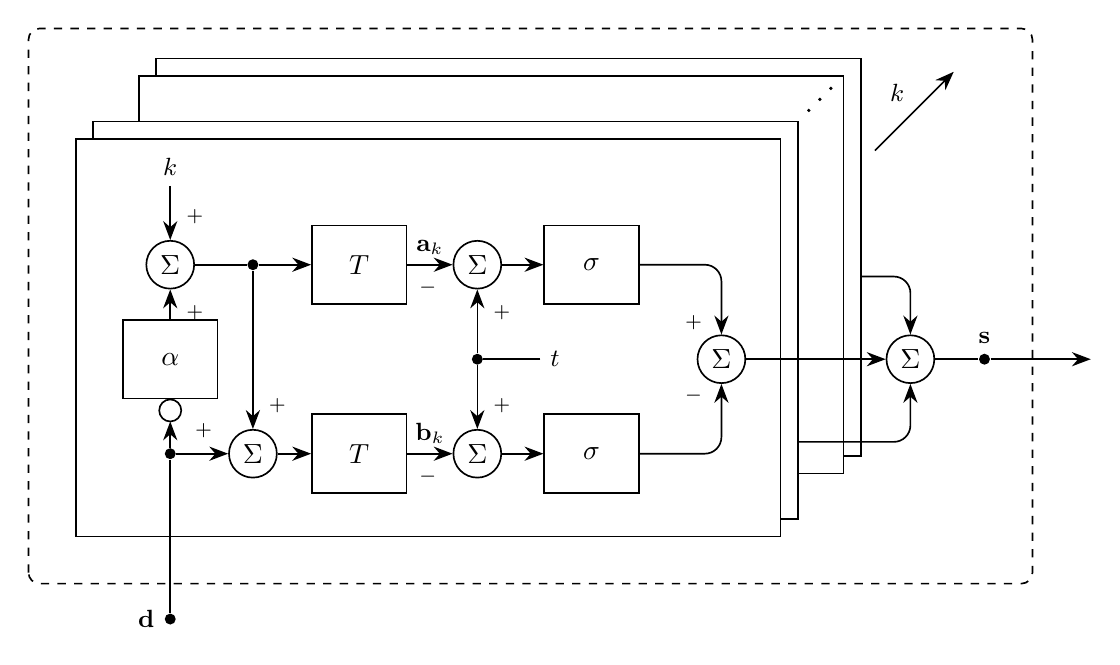
\begin{tikzpicture}[emt diagram]

% Duty and alignment remain dimensionless until the final edge-time gains.
\node[signal, label={[sig]left:$\mathbf{d}$}] (d) at (3.2,-3.3) {};
\node[signal] (split) at (3.2,-\edgerow) {};
\draw[line] (d) -- (split);

% The hollow input bubble complements duty before applying the alignment gain.
\node[block, minimum width=1.2cm] (align) at (3.2,0) {$\alpha$};
\node[draw, semithick, circle, fill=white, inner sep=0pt, outer sep=0pt,
      minimum size=2.8mm, anchor=north] (complement) at (align.south) {};
\draw[->, line] (split) -- (complement.south);

% Each stacked branch constructs its two edge positions within carrier periods.
\node[sum] (on) at (3.2,\edgerow) {$\Sigma$};
\draw[->, line] (align.north) -- (on.south);
\node[pm, anchor=north west] at ($(on.south)+(0.08,-0.08)$) {$+$};
\draw[->, line] (3.2,2.2) node[sig, above] {$k$} -- (on.north);
\node[pm, anchor=south west] at ($(on.north)+(0.08,0.08)$) {$+$};

\node[signal] (edge) at (4.25,\edgerow) {};
\draw[line] (on.east) -- (edge);
\node[sum] (off) at (4.25,-\edgerow) {$\Sigma$};
\draw[->, line] (edge) -- (off.north);
\node[pm, anchor=south west] at ($(off.north)+(0.08,0.08)$) {$+$};
\draw[->, line] (split) -- (off.west);
\node[pm, anchor=south east] at ($(off.west)+(-0.08,0.08)$) {$+$};

% Convert each edge position to time, then subtract it from the current time.
\node[block, minimum width=1.2cm] (ontime) at (5.6,\edgerow) {$T$};
\node[block, minimum width=1.2cm] (offtime) at (5.6,-\edgerow) {$T$};
\draw[->, line] (edge) -- (ontime.west);
\draw[->, line] (off.east) -- (offtime.west);
\node[sum] (risetime) at (7.1,\edgerow) {$\Sigma$};
\node[sum] (falltime) at (7.1,-\edgerow) {$\Sigma$};
\draw[->, line] (ontime.east) -- (risetime.west)
    node[sig, midway, above] {$\mathbf{a}_k$};
\draw[->, line] (offtime.east) -- (falltime.west)
    node[sig, midway, above] {$\mathbf{b}_k$};
\node[pm, anchor=north east] at ($(risetime.west)+(-0.08,-0.08)$) {$-$};
\node[pm, anchor=north east] at ($(falltime.west)+(-0.08,-0.08)$) {$-$};
\node[signal] (time) at (7.1,0) {};
\draw[line] (7.9,0) node[sig, right] {$t$} -- (time);
\draw[->, line] (time) -- (risetime.south);
\draw[->, line] (time) -- (falltime.north);
\node[pm, anchor=north west] at ($(risetime.south)+(0.08,-0.08)$) {$+$};
\node[pm, anchor=south west] at ($(falltime.north)+(0.08,0.08)$) {$+$};

\node[block, minimum width=1.2cm] (rise) at (8.55,\edgerow) {$\sigma$};
\node[block, minimum width=1.2cm] (fall) at (8.55,-\edgerow) {$\sigma$};
\draw[->, line] (risetime.east) -- (rise.west);
\draw[->, line] (falltime.east) -- (fall.west);

% One pulse is the edge difference; all carrier periods contribute.
\node[sum] (pulse) at (10.2,0) {$\Sigma$};
\draw[->, line] (rise.east) -| (pulse.north);
\draw[->, line] (fall.east) -| (pulse.south);
\node[pm, anchor=east] at ($(pulse.north)+(-0.12,0.15)$) {$+$};
\node[pm, anchor=east] at ($(pulse.south)+(-0.12,-0.15)$) {$-$};

\node[sum] (periods) at (12.6,0) {$\Sigma$};
\draw[->, line] (pulse.east) -- (periods.west);
\draw[->, line] (10.95+\stackfar+\stackstep,\outputrow) -| (periods.north);
\draw[->, line] (10.95+\stackstep,-\outputrow) -| (periods.south);
\node[signal, label={[sig]above:$\mathbf{s}$}, right=0.55cm of periods] (s) {};
\draw[line] (periods.east) -- (s);
\draw[->, line] (s) -- ++(1.35,0);

% The stack continues along the carrier-period index.
\draw[->, line] (12.15,2.65) -- (13.15,3.65)
    node[sig, midway, above left] {$k$};
\foreach \offset in {0.36,0.5,0.64}
    \fill (10.95+\offset,2.8+\offset) circle (0.65pt);

\begin{scope}[on background layer]
    \draw[enclosure] (1.4,-2.85) rectangle (14.15,4.2);
    \foreach \offset in {\stackfar+\stackstep,\stackfar,\stackstep,0} {
        \draw[semithick, fill=white]
            (2.0+\offset,-2.25+\offset)
            rectangle (10.95+\offset,2.8+\offset);
    }
\end{scope}

\end{tikzpicture}
\end{document}
